\section{2015 Applied \& Computational Mathematics}

\subsection{Individual}

\begin{exercise}
\label{applied:2015:1}
Let $r$ and $s$ be relatively prime positive integers. Prove that the number of lattice paths from $(0,0)$ to $(r,s)$, consisting of steps $(1,0)$ and $(0,1)$ and never going above the line $ry=sx$, is given by
\[
\frac{1}{r+s}\binom{r+s}{s}.
\]
\end{exercise}

\begin{lemma}[Cycle Lemma]
For any sequence of $r$ horizontal steps $(1,0)$ and $s$ vertical steps $(0,1)$ such that $\gcd(r,s)=1$, exactly one of the $r+s$ cyclic shifts of the sequence generates a lattice path from $(0,0)$ to $(r,s)$ that stays non-strictly below the line $ry=sx$.
\end{lemma}

\begin{solution}
This problem is a classic application of the \textbf{Cycle Lemma} (or Dvoretzky-Motzkin Cycle Lemma), which is a generalization of Bertrand's Ballot Theorem.

Let a path be represented by a sequence of $r+s$ steps $X = (x_1, x_2, \dots, x_{r+s})$, where each $x_i \in \{ (1,0), (0,1) \}$. There are exactly $r$ steps of type $(1,0)$ and $s$ steps of type $(0,1)$. The total number of such sequences is $\binom{r+s}{s}$.

Since $\gcd(r,s)=1$, the line $y = \frac{s}{r}x$ passes through no lattice points between the origin $(0,0)$ and the destination $(r,s)$. The condition that a path never goes above the line $ry=sx$ corresponds to the condition $y_j \leq \frac{s}{r} x_j$ for all $j=1, \dots, r+s$, where $(x_j, y_j)$ is the position after $j$ steps.

Consider the set of all $r+s$ cyclic shifts of a given sequence $X$. Because $\gcd(r,s)=1$, the sequence is not periodic with any period less than $r+s$, so all $r+s$ cyclic shifts are distinct. The Cycle Lemma\footnote{Bertrand's Ballot Theorem is the special case where $r=n$ and $s=k$ with $n > k$, often stated as the probability that one candidate stays strictly ahead of another during a vote count being $\frac{n-k}{n+k}$.} states that for any sequence of $r$ horizontal and $s$ vertical steps where $\gcd(r,s)=1$, exactly one of its $r+s$ cyclic shifts generates a path that stays non-strictly below the line $ry=sx$ (starting from the origin).

Specifically, if we partition the $\binom{r+s}{s}$ total paths into equivalence classes under cyclic shifts\sidenote{To see why exactly one shift works, imagine an infinite "staircase" path formed by concatenating the sequence $X$ repeatedly. The line $y = \frac{s}{r}x$ represents the average direction. Since $\gcd(r,s)=1$, the "lowest" points of the path relative to this average direction occur exactly once per period. Starting the path at this unique global minimum ensures it never drifts above the line in that period.}, each class contains exactly $r+s$ paths, and exactly one path in each class satisfies the "never above" condition. Therefore, the number of such paths is
\[
\frac{1}{r+s} \binom{r+s}{s}.
\]
\end{solution}

\begin{exercise}
\label{applied:2015:2}
The $2\times 2$ block matrix
\[
C(\alpha)=\begin{bmatrix}\alpha I&A\\A^{T}&0\end{bmatrix}
\]
plays a key role in an augmented system method to solve linear least squares problem, a fundamental numerical linear algebra problem for fitting a linear model to observations subject to errors in science, where $A\in\mathbb{R}^{m\times n}$ has full rank $n\leq m$, $I$ is a $m\times m$ identity matrix, and $\alpha\geq 0$.

\begin{enumerate}
\item[(a)] The eigenvalues of $C(\alpha)$ are:
\[
\frac{\alpha}{2}\pm\left(\frac{\alpha^{2}}{4}+\sigma_{i}^{2}\right)^{1/2}\ \mathrm{for}\ i=1,2,\dots,n,\ \mathrm{and}\ \alpha\ (m-n\ \mathrm{times}),
\]
where $\sigma_{i}$ are singular values of $A$ arranged in decreasing order $\sigma_{1}\geq\sigma_{2}\geq\dots\geq\sigma_{n}$.
\item[(b)] The condition number $\kappa_{2}(C(\alpha))=\|C(\alpha)\|_{2} \|[C(\alpha)]^{-1}\|_{2}$ has bounds:
\[
\sqrt{2}\kappa_{2}(A)\leq\min_{\alpha}\kappa_{2}(C(\alpha))\leq 2\kappa_{2}(A),
\]
with $\min_{\alpha}\kappa_{2}(C(\alpha))$ achieved for $\alpha=\sigma_{n}/\sqrt{2}$, and
\[
\max_{\alpha}\kappa_{2}(C(\alpha))>\kappa_{2}(A)^{2}.
\]
\end{enumerate}
\end{exercise}

\textbf{Prerequisites / Core Concepts:}
\begin{itemize}
    \item \textbf{Spectral Condition Number ($\kappa_2$):} For a square non-singular matrix $M$, the condition number in the $L^2$ norm is defined as $\kappa_2(M) = \|M\|_2 \|M^{-1}\|_2$. This is equal to the ratio of the largest to smallest singular value: $\sigma_1(M) / \sigma_n(M)$.
    \item \textbf{Rectangular Condition Number:} For an $m \times n$ matrix $A$ of full rank $n \leq m$, the condition number is generalized as $\kappa_2(A) = \sigma_1(A) / \sigma_n(A)$.
    \item \textbf{Spectral Norm ($\|\cdot\|_2$):} The matrix norm induced by the Euclidean vector norm. For any matrix $M$, $\|M\|_2 = \sigma_{\max}(M)$. If $M$ is symmetric, $\|M\|_2 = \max_i |\lambda_i|$.
\end{itemize}

\begin{solution}
\textbf{(a)} Let $\lambda$ be an eigenvalue of $C(\alpha)$ with eigenvector $\begin{bmatrix} x \\ y \end{bmatrix}$, where $x \in \mathbb{R}^m$ and $y \in \mathbb{R}^n$. The eigenvalue equation is:
\begin{align}
    \alpha x + Ay &= \lambda x \label{eq:eig1} \\
    A^T x &= \lambda y \label{eq:eig2}
\end{align}
\textbf{Case 1:} $\lambda = \alpha$. From \eqref{eq:eig1}, $Ay = 0$. Since $A$ has full rank $n$, we must have $y=0$. Then \eqref{eq:eig2} implies $A^T x = 0$. The dimension of $\text{null}(A^T)$ is $m-n$. Thus, $\lambda = \alpha$ is an eigenvalue with multiplicity $m-n$.

\textbf{Case 2:} $\lambda \neq \alpha$. From \eqref{eq:eig1}, $x = \frac{1}{\lambda - \alpha} Ay$. Substituting this into \eqref{eq:eig2}:
\[
A^T \left( \frac{1}{\lambda - \alpha} Ay \right) = \lambda y \implies A^T A y = \lambda(\lambda - \alpha) y.
\]
The eigenvalues of $A^T A$ are $\sigma_i^2$ for $i=1, \dots, n$. Thus:
\[
\lambda^2 - \alpha \lambda - \sigma_i^2 = 0 \implies \lambda = \frac{\alpha \pm \sqrt{\alpha^2 + 4\sigma_i^2}}{2}.
\]
This gives $2n$ eigenvalues. Combined with the $m-n$ eigenvalues from Case 1, we have a total of $m+n$ eigenvalues.

\textbf{(b) Detailed Analysis of the Condition Number}

\begin{enumerate}
    \item \textbf{Step 1: Singular Values and the Condition Number.}
    The matrix $C(\alpha)$ is symmetric, so its singular values $\sigma_i(C(\alpha))$ are the absolute values of its eigenvalues. From part (a), the eigenvalues are:
    \begin{itemize}
        \item $\lambda_i^{+} = \frac{\alpha}{2} + \sqrt{\frac{\alpha^2}{4} + \sigma_i^2}$ for $i=1, \dots, n$. (These are always positive for $\alpha \ge 0, \sigma_i > 0$)
        \item $\lambda_i^{-} = \frac{\alpha}{2} - \sqrt{\frac{\alpha^2}{4} + \sigma_i^2}$ for $i=1, \dots, n$. (These are always negative)
        \item $\lambda_0 = \alpha$ (with multiplicity $m-n$).
    \end{itemize}
    The condition number is defined as $\kappa_2(C(\alpha)) = \frac{\sigma_{\max}(C(\alpha))}{\sigma_{\min}(C(\alpha))}$. Our goal is to find the minimum of this value with respect to $\alpha$.

    \item \textbf{Step 2: Finding the Maximum Singular Value.}
    The singular values are the magnitudes of the eigenvalues. Since $\sigma_1 \ge \sigma_2 \ge \dots \ge \sigma_n > 0$:
    \[ \sigma_{\max}(C(\alpha)) = \max_i |\lambda_i^{\pm}|, |\lambda_0| \]
    The largest eigenvalue is clearly $\lambda_1^{+} = \frac{\alpha}{2} + \sqrt{\frac{\alpha^2}{4} + \sigma_1^2}$. This value is positive, so its magnitude is itself. Let's call this $f(\alpha)$.
    \[ \sigma_{\max}(C(\alpha)) = f(\alpha) = \frac{\alpha + \sqrt{\alpha^2 + 4\sigma_1^2}}{2}. \]

    \item \textbf{Step 3: Finding the Minimum Singular Value.}
    The minimum singular value is the minimum of all the magnitudes.
    \[ \sigma_{\min}(C(\alpha)) = \min \left( \min_{i} |\lambda_i^{+}|, \min_{i} |\lambda_i^{-}|, |\lambda_0| \right) \]
    \begin{itemize}
        \item For $|\lambda_i^{+}|$: The minimum occurs at $i=n$, giving $\frac{\alpha}{2} + \sqrt{\frac{\alpha^2}{4} + \sigma_n^2}$.
        \item For $|\lambda_i^{-}|$: The magnitude is $|\frac{\alpha}{2} - \sqrt{\frac{\alpha^2}{4} + \sigma_i^2}| = \sqrt{\frac{\alpha^2}{4} + \sigma_i^2} - \frac{\alpha}{2}$. The minimum of this expression occurs when $\sigma_i$ is smallest, i.e., at $i=n$. This gives $\sqrt{\frac{\alpha^2}{4} + \sigma_n^2} - \frac{\alpha}{2}$. Let's call this $g(\alpha) = \frac{\sqrt{\alpha^2+4\sigma_n^2}-\alpha}{2}$.
        \item For $|\lambda_0|$: The magnitude is simply $\alpha$.
    \end{itemize}
    Comparing these minimums, $\frac{\alpha}{2} + \sqrt{\frac{\alpha^2}{4} + \sigma_n^2}$ is clearly larger than both $\alpha$ and $g(\alpha)$. So we only need to compare $\alpha$ and $g(\alpha)$.
    \[ \sigma_{\min}(C(\alpha)) = \min\{\alpha, g(\alpha)\}. \]

    \item \textbf{Step 4: Minimizing the Condition Number.}
    The condition number is $\kappa_2(C(\alpha)) = \frac{f(\alpha)}{\min\{\alpha, g(\alpha)\}}$. To minimize this fraction, we want to maximize the denominator.
    Let's analyze the functions in the denominator: $y_1(\alpha) = \alpha$ is strictly increasing. For $y_2(\alpha) = g(\alpha)$, its derivative is $g'(\alpha) = \frac{1}{2}(\frac{\alpha}{\sqrt{\alpha^2+4\sigma_n^2}}-1)$, which is always negative because $\sqrt{\alpha^2+4\sigma_n^2} > \alpha$. So $g(\alpha)$ is strictly decreasing.
    The function $\min\{\alpha, g(\alpha)\}$ will be maximized at the point where $\alpha = g(\alpha)$.
    
    Solving for this optimal $\alpha$:
    \begin{align*}
    \alpha &= \frac{\sqrt{\alpha^2 + 4\sigma_n^2} - \alpha}{2} \\
    2\alpha &= \sqrt{\alpha^2 + 4\sigma_n^2} - \alpha \\
    3\alpha &= \sqrt{\alpha^2 + 4\sigma_n^2} \\
    (3\alpha)^2 &= \alpha^2 + 4\sigma_n^2 \quad (\text{squaring both sides}) \\
    9\alpha^2 &= \alpha^2 + 4\sigma_n^2 \\
    8\alpha^2 &= 4\sigma_n^2 \\
    \alpha^2 &= \frac{\sigma_n^2}{2} \implies \alpha = \frac{\sigma_n}{\sqrt{2}}.
    \end{align*}

    \item \textbf{Step 5: Calculating the Minimum Condition Number.}
    At this optimal value $\alpha = \sigma_n/\sqrt{2}$, the denominator is $\sigma_n/\sqrt{2}$. The numerator is:
    \[ f(\sigma_n/\sqrt{2}) = \frac{\sigma_n/\sqrt{2} + \sqrt{(\sigma_n/\sqrt{2})^2 + 4\sigma_1^2}}{2} = \frac{\sigma_n/\sqrt{2} + \sqrt{\sigma_n^2/2 + 4\sigma_1^2}}{2}. \]
    The condition number is then:
    \begin{align*}
    \kappa_2(C(\alpha_{opt})) &= \frac{\frac{\sigma_n/\sqrt{2} + \sqrt{\sigma_n^2/2 + 4\sigma_1^2}}{2}}{\sigma_n/\sqrt{2}} \\
    &= \frac{1}{2} + \frac{\sqrt{\sigma_n^2/2 + 4\sigma_1^2}}{2(\sigma_n/\sqrt{2})} \\
    &= \frac{1}{2} + \frac{\sqrt{\sigma_n^2/2 + 4\sigma_1^2}}{\sqrt{2}\sigma_n} \\
    &= \frac{1}{2} + \sqrt{\frac{\sigma_n^2/2 + 4\sigma_1^2}{2\sigma_n^2}} \\
    &= \frac{1}{2} + \sqrt{\frac{1}{4} + \frac{4\sigma_1^2}{2\sigma_n^2}} \\
    &= \frac{1}{2} + \sqrt{\frac{1}{4} + 2\left(\frac{\sigma_1}{\sigma_n}\right)^2}.
    \end{align*}
    Since the condition number of A is $\kappa_2(A) = \sigma_1/\sigma_n$, we get the final expression:
    \[ \min_{\alpha}\kappa_2(C(\alpha)) = \frac{1}{2} + \sqrt{\frac{1}{4} + 2\kappa_2(A)^2}. \]

    \item \textbf{Step 6: Verifying the Bounds.}
    Let $K = \kappa_2(A) \ge 1$. We need to prove $\sqrt{2}K \le \frac{1}{2} + \sqrt{\frac{1}{4} + 2K^2} \le 2K$.
    \begin{itemize}
        \item \textbf{Upper Bound:} $\frac{1}{2} + \sqrt{\frac{1}{4} + 2K^2} \le 2K$.
        \[ \sqrt{\frac{1}{4} + 2K^2} \le 2K - \frac{1}{2}. \]
        Since $K \ge 1$, the right side is positive, so we can square both sides:
        \[ \frac{1}{4} + 2K^2 \le \left(2K - \frac{1}{2}\right)^2 = 4K^2 - 2K + \frac{1}{4}. \]
        \[ 0 \le 2K^2 - 2K = 2K(K-1). \]
        This is true for all $K \ge 1$.
        \item \textbf{Lower Bound:} $\sqrt{2}K \le \frac{1}{2} + \sqrt{\frac{1}{4} + 2K^2}$.
        \[ \sqrt{2}K - \frac{1}{2} \le \sqrt{\frac{1}{4} + 2K^2}. \]
        Since $K \ge 1$, the left side is positive, so we can square both sides:
        \[ (\sqrt{2}K - \frac{1}{2})^2 \le \frac{1}{4} + 2K^2. \]
        \[ 2K^2 - \sqrt{2}K + \frac{1}{4} \le \frac{1}{4} + 2K^2. \]
        \[ -\sqrt{2}K \le 0. \]
        This is true for all $K \ge 1$. Both bounds hold.
    \end{itemize}

    \item \textbf{Step 7: Verifying the Maximum Behavior.}
    The problem states $\max_{\alpha}\kappa_{2}(C(\alpha))>\kappa_{2}(A)^{2}$.
    As shown, $\kappa_2(C(\alpha)) = \frac{f(\alpha)}{\min\{\alpha, g(\alpha)\}}$.
    Let's analyze the behavior for large $\alpha$:
    \begin{itemize}
        \item $f(\alpha) = \frac{\alpha}{2} + \sqrt{\frac{\alpha^2}{4} + \sigma_1^2} = \frac{\alpha}{2} + \frac{\alpha}{2}\sqrt{1 + \frac{4\sigma_1^2}{\alpha^2}} \approx \frac{\alpha}{2} + \frac{\alpha}{2}\left(1 + \frac{2\sigma_1^2}{\alpha^2}\right) = \alpha + \frac{\sigma_1^2}{\alpha}$.
        \item $g(\alpha) = \frac{\sqrt{\alpha^2 + 4\sigma_n^2} - \alpha}{2} = \frac{\alpha\sqrt{1 + 4\sigma_n^2/\alpha^2} - \alpha}{2} \approx \frac{\alpha(1 + 2\sigma_n^2/\alpha^2) - \alpha}{2} = \frac{\sigma_n^2}{\alpha}$.
    \end{itemize}
    For large $\alpha$, $g(\alpha) \approx \sigma_n^2/\alpha$ will be much smaller than $\alpha$, so $\min\{\alpha, g(\alpha)\} = g(\alpha)$.
    The condition number becomes:
    \[ \kappa_2(C(\alpha)) \approx \frac{\alpha + \sigma_1^2/\alpha}{\sigma_n^2/\alpha} = \frac{\alpha^2 + \sigma_1^2}{\sigma_n^2} = \frac{\alpha^2}{\sigma_n^2} + \left(\frac{\sigma_1}{\sigma_n}\right)^2 = \frac{\alpha^2}{\sigma_n^2} + \kappa_2(A)^2. \]
    Since we can choose $\alpha$ to be arbitrarily large, the condition number can be made arbitrarily large. Thus, $\max_{\alpha} \kappa_2(C(\alpha))$ is unbounded, and it is certainly greater than $\kappa_2(A)^2$.
\end{enumerate}
\end{solution}

\begin{exercise}
\label{applied:2015:3}
Solve the linear hyperbolic PDE:
\begin{equation}
u_{t}+au_{x}=0,\quad t\geq 0, \tag{1}
\end{equation}
where $a$ is constant. Using the finite difference approximation:
\begin{equation}
\frac{u_{m}^{n+1}-u_{m}^{n}}{k}+a\frac{u_{m+1}^{n}-u_{m-1}^{n}}{2h}=0, \tag{2}
\end{equation}
where $k$ and $h$ are temporal and spatial mesh sizes.

\begin{enumerate}
\item[(a)] Show that when $\lambda=k/h$ is fixed as a positive constant, the forward-time central-space scheme is consistent with the equation.
\item[(b)] Analyze stability. Is the method stable with $\lambda=k/h$ fixed as constant?
\item[(c)] How would the answer change if $\lambda=k/h$ can be made small?
\item[(d)] Would this be a good scheme to use even if you can make it stable by making $\lambda$ small? If not, provide a simple modification to make the scheme stable while keeping $\lambda$ fixed.
\end{enumerate}
\end{exercise}

\begin{solution}
\begin{solution}
This exercise analyzes the consistency and stability of the standard Forward-Time Central-Space (FTCS) finite difference scheme for the 1D linear advection equation, a canonical hyperbolic PDE.

\textbf{The Advection Equation and its Solution}
The equation $u_t + a u_x = 0$ describes a wave profile that travels with constant velocity $a$ without changing its shape. Given an initial condition $u(x,0) = f(x)$, the exact solution is $u(x,t) = f(x-at)$. This is found using the method of characteristics, where we observe that the solution is constant along the lines $x - at = \text{const}$.

\textbf{(a) Consistency of the FTCS Scheme}
Consistency means that in the limit as the mesh sizes $k$ (time step) and $h$ (space step) go to zero, the finite difference equation should become identical to the original PDE. To show this, we perform a Taylor series expansion of each term in the scheme around the point $(x_m, t_n)$, where $u_m^n = u(x_m, t_n)$.

\begin{enumerate}
    \item \textbf{Taylor Expansions:}
    The term $u_m^{n+1}$ is expanded in time:
    \[ u_m^{n+1} = u(x_m, t_n+k) = u(x_m, t_n) + k \frac{\partial u}{\partial t} + \frac{k^2}{2} \frac{\partial^2 u}{\partial t^2} + O(k^3). \]
    The terms $u_{m\pm 1}^n$ are expanded in space:
    \[ u_{m+1}^n = u(x_m+h, t_n) = u(x_m, t_n) + h \frac{\partial u}{\partial x} + \frac{h^2}{2} \frac{\partial^2 u}{\partial x^2} + \frac{h^3}{6} \frac{\partial^3 u}{\partial x^3} + O(h^4). \]
    \[ u_{m-1}^n = u(x_m-h, t_n) = u(x_m, t_n) - h \frac{\partial u}{\partial x} + \frac{h^2}{2} \frac{\partial^2 u}{\partial x^2} - \frac{h^3}{6} \frac{\partial^3 u}{\partial x^3} + O(h^4). \]
    
    \item \textbf{Approximating the Derivatives:}
    From these expansions, we can see how the finite differences approximate the true derivatives:
    \begin{itemize}
        \item \textbf{Time Derivative:} $\frac{u_m^{n+1} - u_m^n}{k} = \frac{\partial u}{\partial t} + \frac{k}{2} \frac{\partial^2 u}{\partial t^2} + O(k^2)$.
        \item \textbf{Space Derivative:} $\frac{u_{m+1}^n - u_{m-1}^n}{2h} = \frac{(u+h u_x + \dots) - (u-h u_x + \dots)}{2h} = \frac{2h u_x + \frac{h^3}{3}u_{xxx} + O(h^5)}{2h} = \frac{\partial u}{\partial x} + \frac{h^2}{6} \frac{\partial^3 u}{\partial x^3} + O(h^4)$.
    \end{itemize}
    
    \item \textbf{Substituting into the Scheme:}
    Plugging these approximations into the finite difference scheme gives:
    \[ \left( u_t + \frac{k}{2} u_{tt} + O(k^2) \right) + a \left( u_x + \frac{h^2}{6} u_{xxx} + O(h^4) \right) = 0. \]
    Rearranging this equation isolates the original PDE:
    \[ (u_t + a u_x) + \left( \frac{k}{2} u_{tt} + a \frac{h^2}{6} u_{xxx} + \dots \right) = 0. \]
    
    \item \textbf{Local Truncation Error (LTE):}
    The Local Truncation Error, $\tau$, is the amount by which the exact solution fails to satisfy the discrete equation. It is the second term in the expression above:
    \[ \tau = \frac{k}{2} u_{tt} + a \frac{h^2}{6} u_{xxx} + \dots \]
    The scheme is said to be consistent if $\tau \to 0$ as $k, h \to 0$. Since the lowest powers of $k$ and $h$ in $\tau$ are $k^1$ and $h^2$, the scheme is first-order in time and second-order in space, written as $O(k, h^2)$. As $k,h \to 0$, the truncation error vanishes. Therefore, the FTCS scheme is consistent with the advection equation.
\end{enumerate}

\textbf{(b) Stability Analysis}
We use Von Neumann stability analysis to determine if errors are amplified or damped over time. We test the scheme with a single Fourier mode ansatz, $u_m^n = G^n(\theta) e^{i(m\theta)}$, where $\theta = \xi h$ is the dimensionless wave number and $G(\theta)$ is the amplification factor per time step for that mode. For a stable scheme, we require $|G(\theta)| \le 1$ for all $\theta$.

\begin{enumerate}
    \item \textbf{Substitute the Ansatz:}
    The scheme is $\frac{u_{m}^{n+1}-u_{m}^{n}}{k}+a\frac{u_{m+1}^{n}-u_{m-1}^{n}}{2h}=0$. Substituting $u_m^n = G^n e^{im\theta}$:
    \[ \frac{G^{n+1}e^{im\theta} - G^n e^{im\theta}}{k} + a \frac{G^n e^{i(m+1)\theta} - G^n e^{i(m-1)\theta}}{2h} = 0. \]
    
    \item \textbf{Solve for the Amplification Factor G:}
    Divide the entire equation by the common factor $G^n e^{im\theta}$:
    \[ \frac{G - 1}{k} + a \frac{e^{i\theta} - e^{-i\theta}}{2h} = 0. \]
    Let $\lambda = k/h$ (the Courant number). Rearranging for $G$:
    \[ G = 1 - \frac{ak}{2h} (e^{i\theta} - e^{-i\theta}) = 1 - \frac{a\lambda}{2} (2i \sin\theta) = 1 - i a \lambda \sin\theta. \]
    
    \item \textbf{Analyze the Magnitude of G:}
    The magnitude squared of the amplification factor is:
    \[ |G|^2 = (\text{Re}(G))^2 + (\text{Im}(G))^2 = (1)^2 + (-a\lambda\sin\theta)^2 = 1 + (a\lambda\sin\theta)^2. \]
    For stability, we require $|G|^2 \le 1$. However, since $a$ is a real constant and $\lambda > 0$, the term $(a\lambda\sin\theta)^2$ is always non-negative.
    \[ |G|^2 = 1 + (a\lambda\sin\theta)^2 \ge 1. \]
    The equality holds only if $\sin\theta=0$ (i.e., for the longest wavelength modes). For any other mode where $\sin\theta \neq 0$, we have $|G|^2 > 1$. This means that almost all Fourier modes of an error will be amplified at every time step, leading to exponential growth.
    
    \textbf{Conclusion:} The scheme is \textbf{unconditionally unstable} for any fixed $\lambda > 0$.

\end{enumerate}

\textbf{(c) Conditional Stability}
The question asks what happens if $\lambda=k/h$ can be made small. This typically implies a different scaling relationship between $k$ and $h$. The strict condition for stability is $|G| \leq 1$. As we've shown, this is never met.

However, a weaker form of stability (sometimes called practical stability for a finite time $T$) requires that the total amplification over a fixed time interval remains bounded. The number of steps is $N = T/k$. We need $|G|^N$ to be bounded.
\[ |G|^N = \left(\sqrt{1 + (a\lambda\sin\theta)^2}\right)^{T/k} = \left(1 + a^2\lambda^2\sin^2\theta\right)^{T/(2k)}. \]
Using the approximation $(1+x)^p \approx e^{px}$ for small $x$:
\[ |G|^N \approx \exp\left( \frac{T}{2k} a^2 \lambda^2 \sin^2\theta \right) = \exp\left( \frac{T}{2k} a^2 \frac{k^2}{h^2} \sin^2\theta \right) = \exp\left( T \frac{a^2 k}{2h^2} \sin^2\theta \right). \]
For this amplification to remain bounded as $k,h \to 0$, we need the exponent to be bounded. This requires the ratio $\frac{k}{h^2}$ to be held constant.
So, if we can make $\lambda = k/h$ small by choosing a time step $k$ that is on the order of $h^2$ (i.e., $k = C h^2$ for some constant $C$), then the scheme becomes stable. This is known as a \textbf{diffusive stability limit}, and it is generally too restrictive for hyperbolic problems.

\textbf{(d) A Better Scheme: Lax-Friedrichs}
The FTCS scheme is a poor choice because it is unconditionally unstable under the standard hyperbolic scaling $k=O(h)$. This instability arises because the central difference for the spatial derivative is not "aware" of the direction of wave propagation.

A simple modification to achieve stability is the \textbf{Lax-Friedrichs scheme}. It replaces the term $u_m^n$ in the time-stepping with the average of its spatial neighbors, $\frac{1}{2}(u_{m+1}^n + u_{m-1}^n)$. This explicitly introduces numerical diffusion.

The modified scheme is:
\[ \frac{u_m^{n+1} - \frac{1}{2}(u_{m+1}^n + u_{m-1}^n)}{k} + a\frac{u_{m+1}^n - u_{m-1}^n}{2h} = 0. \]
Let's analyze its stability with the same Von Neumann method.
\begin{enumerate}
    \item \textbf{Substitute the Ansatz:}
    \[ \frac{G^{n+1}e^{im\theta} - \frac{1}{2}(G^n e^{i(m+1)\theta} + G^n e^{i(m-1)\theta})}{k} + a\frac{G^n e^{i(m+1)\theta} - G^n e^{i(m-1)\theta}}{2h} = 0. \]
    
    \item \textbf{Solve for G:} Divide by $G^n e^{im\theta}$:
    \[ \frac{G - \frac{1}{2}(e^{i\theta} + e^{-i\theta})}{k} + a\frac{e^{i\theta} - e^{-i\theta}}{2h} = 0. \]
    Using $e^{i\theta} + e^{-i\theta} = 2\cos\theta$ and $e^{i\theta} - e^{-i\theta} = 2i\sin\theta$:
    \[ \frac{G - \cos\theta}{k} + a\frac{2i\sin\theta}{2h} = 0. \]
    \[ G = \cos\theta - \frac{iak}{h}\sin\theta = \cos\theta - ia\lambda\sin\theta. \]
    
    \item \textbf{Analyze the Magnitude:}
    \[ |G|^2 = (\cos\theta)^2 + (-a\lambda\sin\theta)^2 = \cos^2\theta + (a\lambda)^2\sin^2\theta. \]
    For stability, we need $|G|^2 \le 1$:
    \[ \cos^2\theta + (a\lambda)^2\sin^2\theta \le 1. \]
    Using $\cos^2\theta = 1 - \sin^2\theta$:
    \[ 1 - \sin^2\theta + (a\lambda)^2\sin^2\theta \le 1. \]
    \[ ((a\lambda)^2 - 1)\sin^2\theta \le 0. \]
    Since $\sin^2\theta \ge 0$, this inequality holds if and only if $(a\lambda)^2 - 1 \le 0$.
    \[ (a\lambda)^2 \le 1 \implies |a\lambda| \le 1. \]
    
    \textbf{Conclusion:} The Lax-Friedrichs scheme is stable provided the Courant-Friedrichs-Lewy (CFL) condition $|a| \frac{k}{h} \le 1$ is satisfied. This is a much more practical condition than $k=O(h^2)$, making it a good, simple, stable scheme for this equation.
\end{enumerate}
\end{solution}
\end{solution}

\begin{exercise}
\label{applied:2015:4}
Let $A,H,Q\in\mathbb{C}^{n\times n} and $Q$ is nonsingular. Assume $H=Q^{-1}AQ$ and $H$ is properly upper Hessenberg. Show that
\[
\mathrm{span}\{q_{1},q_{2},\dots,q_{j}\}=\mathcal{K}_{j}(A,q_{1}),\quad j=1,2,\dots,n,
\]
where $q_{j}$ is the $j$-th column of $Q$, and $\mathcal{K}_{j}(A,q_{1})=\mathrm{span}\{q_{1},Aq_{1},\dots,A^{j-1}q_{1}\}$.
\end{exercise}

\begin{solution}
This is a fundamental result connecting matrix similarity transformations to Krylov subspaces. It forms the basis of the Arnoldi iteration, which is a key algorithm for finding eigenvalues of large matrices. We will prove the statement by induction on $j$.

\textbf{Step 1: Unpacking the Matrix Equation}
The given relation is $H = Q^{-1}AQ$. Pre-multiplying by $Q$ gives us the more convenient form:
\[ AQ = QH \]
Let's write this out by showing the columns of $Q = [q_1, q_2, \dots, q_n]$ and the entries of $H = (h_{ij})$:
\[ A[q_1, q_2, \dots, q_n] = [q_1, q_2, \dots, q_n] \begin{pmatrix}
h_{11} & h_{12} & \cdots & h_{1n} \\
h_{21} & h_{22} & \cdots & h_{2n} \\
0 & h_{32} & \cdots & h_{3n} \\
\vdots & \ddots & \ddots & \vdots \\
0 & \cdots & 0 & h_{n,n-1} & h_{nn}
\end{pmatrix} \]
By considering the $j$-th column of this matrix equation, we get the relationship between $Aq_j$ and the columns of $Q$:
\[ A q_j = \sum_{i=1}^n q_i h_{ij}. \]

\textbf{Step 2: Applying the Hessenberg Structure}
The matrix $H$ is not a full matrix; it is \textbf{upper Hessenberg}, which means $h_{ij} = 0$ for all $i > j+1$. This dramatically simplifies the sum above. The sum for $Aq_j$ only needs to go up to $i = j+1$:
\[ A q_j = \sum_{i=1}^{j+1} q_i h_{ij} = h_{1j}q_1 + h_{2j}q_2 + \dots + h_{jj}q_j + h_{j+1,j}q_{j+1}. \]
This equation is often called the \textbf{Arnoldi relation}.

Furthermore, $H$ is \textbf{properly} upper Hessenberg. This means that all of its sub-diagonal entries are non-zero: $h_{j+1, j} \neq 0$ for $j=1, \dots, n-1$. This is a crucial property, as it allows us to isolate $q_{j+1}$:
\[ h_{j+1, j} q_{j+1} = A q_j - \sum_{i=1}^j h_{ij} q_i \implies q_{j+1} = \frac{1}{h_{j+1, j}} \left( A q_j - \sum_{i=1}^j h_{ij} q_i \right). \]
This shows that the vector $q_{j+1}$ can be generated from the previous vectors $q_1, \dots, q_j$ and the action of $A$ on $q_j$. This is the heart of the inductive proof.

\textbf{Step 3: Proof by Induction}
We want to prove that $\mathcal{Q}_j := \mathrm{span}\{q_1, \dots, q_j\}$ is equal to the Krylov subspace $\mathcal{K}_j(A, q_1) := \mathrm{span}\{q_1, Aq_1, \dots, A^{j-1}q_1\}$ for all $j=1, \dots, n$.

\textbf{Base Case ($j=1$):}
The statement is $\mathrm{span}\{q_1\} = \mathcal{K}_1(A, q_1)$.
By definition, $\mathcal{K}_1(A, q_1) = \mathrm{span}\{q_1\}$. The base case holds trivially.

\textbf{Inductive Hypothesis:}
Assume that for some $j < n$, the statement is true: $\mathcal{Q}_j = \mathcal{K}_j(A, q_1)$.

\textbf{Inductive Step (Prove for $j+1$):}
We need to prove that $\mathcal{Q}_{j+1} = \mathcal{K}_{j+1}(A, q_1)$. We do this by showing inclusion in both directions.

\begin{enumerate}
    \item[($\subseteq$)] \textbf{Show $\mathcal{Q}_{j+1} \subseteq \mathcal{K}_{j+1}(A, q_1)$.}
    By definition, $\mathcal{Q}_{j+1} = \mathrm{span}\{q_1, \dots, q_j, q_{j+1}\} = \mathcal{Q}_j + \mathrm{span}\{q_{j+1}\}$.
    By the inductive hypothesis, $\mathcal{Q}_j = \mathcal{K}_j(A, q_1)$. Since $\mathcal{K}_j(A, q_1) \subseteq \mathcal{K}_{j+1}(A, q_1)$, we just need to show that the new vector $q_{j+1}$ is also in $\mathcal{K}_{j+1}(A, q_1)$.
    From the rearranged Arnoldi relation:
    \[ q_{j+1} = \frac{1}{h_{j+1, j}} \left( A q_j - \sum_{i=1}^j h_{ij} q_i \right). \]
    Let's analyze the two terms on the right:
    \begin{itemize}
        \item $A q_j$: By the inductive hypothesis, $q_j \in \mathcal{Q}_j = \mathcal{K}_j(A, q_1)$. This means $q_j$ is a linear combination of $\{q_1, \dots, A^{j-1}q_1\}$. Therefore, $Aq_j$ is a linear combination of $\{Aq_1, \dots, A^j q_1\}$, which means $A q_j \in \mathrm{span}\{Aq_1, \dots, A^j q_1\} \subseteq \mathcal{K}_{j+1}(A, q_1)$.
        \item $\sum_{i=1}^j h_{ij} q_i$: This is a linear combination of vectors in $\mathcal{Q}_j$. By the hypothesis, $\mathcal{Q}_j = \mathcal{K}_j(A, q_1) \subseteq \mathcal{K}_{j+1}(A, q_1)$. So this sum is in $\mathcal{K}_{j+1}(A, q_1)$.
    \end{itemize}
    Since $q_{j+1}$ is a linear combination of vectors that are all in $\mathcal{K}_{j+1}(A, q_1)$, it must also be in $\mathcal{K}_{j+1}(A, q_1)$. This proves the first inclusion: $\mathcal{Q}_{j+1} \subseteq \mathcal{K}_{j+1}(A, q_1)$.

    \item[($\supseteq$)] \textbf{Show $\mathcal{K}_{j+1}(A, q_1) \subseteq \mathcal{Q}_{j+1}$.}
    By definition, $\mathcal{K}_{j+1} = \mathcal{K}_j + \mathrm{span}\{A^j q_1\}$.
    By the inductive hypothesis, $\mathcal{K}_j = \mathcal{Q}_j \subseteq \mathcal{Q}_{j+1}$. So we just need to show that the new vector $A^j q_1$ is also in $\mathcal{Q}_{j+1}$.
    From the hypothesis, $q_j \in \mathcal{K}_j = \mathrm{span}\{q_1, \dots, A^{j-1}q_1\}$. We can write $A^{j-1}q_1$ as a linear combination of vectors in $\mathcal{Q}_j$: $A^{j-1}q_1 = \sum_{k=1}^j c_k q_k$.
    Applying $A$ to both sides:
    \[ A^j q_1 = A \left( \sum_{k=1}^j c_k q_k \right) = \sum_{k=1}^j c_k (A q_k). \]
    Now we use the Arnoldi relation again: $Aq_k = \sum_{i=1}^{k+1} h_{ik} q_i$. Since $k \le j$, we know $k+1 \le j+1$. This means every $Aq_k$ is a linear combination of $\{q_1, \dots, q_{j+1}\}$, so $Aq_k \in \mathcal{Q}_{j+1}$.
    Since $A^j q_1$ is a linear combination of vectors $\{Aq_1, \dots, Aq_j\}$, all of which are in $\mathcal{Q}_{j+1}$, it must also be in $\mathcal{Q}_{j+1}$. This proves the second inclusion.
\end{enumerate}

Since we have shown $\mathcal{Q}_{j+1} \subseteq \mathcal{K}_{j+1}(A, q_1)$ and $\mathcal{K}_{j+1}(A, q_1) \subseteq \mathcal{Q}_{j+1}$, the two sets must be equal.

\textbf{Alternative Conclusion via Dimension Counting}
After proving $\mathcal{Q}_{j+1} \subseteq \mathcal{K}_{j+1}(A, q_1)$, we can argue as follows:
\begin{itemize}
    \item The dimension of $\mathcal{Q}_{j+1}$ is $j+1$ because $Q$ is non-singular, meaning its columns $\{q_1, \dots, q_{j+1}\}$ are linearly independent.
    \item The dimension of the Krylov subspace $\mathcal{K}_{j+1}(A, q_1)$ is also $j+1$. This is not always true, but it is guaranteed here because we are given that $H$ is \textit{properly} Hessenberg ($h_{k+1,k} \neq 0$). This "no breakdown" condition in the Arnoldi process ensures that the vectors $\{q_1, Aq_1, \dots, A^j q_1\}$ are linearly independent.
\end{itemize}
Since $\mathcal{Q}_{j+1}$ is a subspace of $\mathcal{K}_{j+1}(A, q_1)$ and they both have the same finite dimension, they must be the same space. This completes the proof.
\end{solution}

\begin{exercise}
\label{applied:2015:5}
[Minkowski Problem]
(see Figure \ref{fig:minkowski}) Assume $P$ is a convex polyhedron embedded in $\mathbb{R}^{3}$ with faces $\{F_{1},F_{2},\cdots,F_{k}\}$. The unit normal vector to face $F_{i}$ is $\mathbf{n}_{i}$ and area is $A_{i}$, $1\leq i\leq k$.

\begin{enumerate}
\item Show that:
\begin{equation}
A_{1}\mathbf{n}_{1}+A_{2}\mathbf{n}_{2}+\dots A_{k}\mathbf{n}_{k}=\mathbf{0}. \tag{3}
\end{equation}
\item Given $k$ unit vectors $\{\mathbf{n}_{1},\mathbf{n}_{2},\dots,\mathbf{n}_{k}\}$ which cannot be contained in any half space, and $k$ positive real numbers $\{A_{1},A_{2},\dots,A_{k}\}$ satisfying condition (3), show that there exists a convex polyhedron $P$ whose face normals are $\mathbf{n}_{i}$ and face areas are $A_{i}$.
\end{enumerate}
\end{exercise}

\begin{center}
  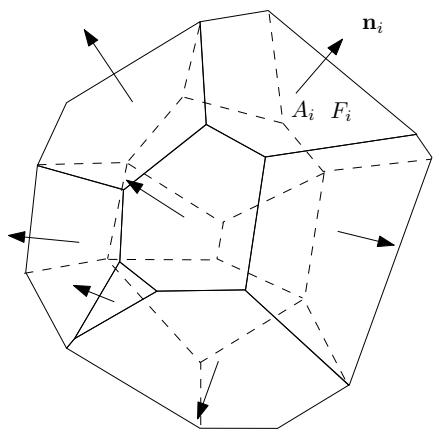
\includegraphics[width=0.7\textwidth]{images/applied/c9aa66d7f3fa71aee892c128f678b8fd0134eeba35d6dff1e42e18157c2c628c.jpg}
  \captionof{figure}{Convex polyhedron with face normals and areas.}
  \label{fig:minkowski}
\end{center}

\begin{solution}
\textbf{1.} Let $\mathbf{c} \in \mathbb{R}^3$ be an arbitrary constant vector. By the Divergence Theorem:
\[
\int_P \nabla \cdot \mathbf{c} \, dV = \oint_{\partial P} \mathbf{c} \cdot \mathbf{n} \, dS.
\]
Since $\mathbf{c}$ is constant, $\nabla \cdot \mathbf{c} = 0$. The boundary $\partial P$ consists of the faces $F_i$ with constant normals $\mathbf{n}_i$. Thus:
\[
0 = \sum_{i=1}^k \int_{F_i} \mathbf{c} \cdot \mathbf{n}_i \, dS = \sum_{i=1}^k (\mathbf{c} \cdot \mathbf{n}_i) A_i = \mathbf{c} \cdot \left( \sum_{i=1}^k A_i \mathbf{n}_i \right).
\]
Since this must hold for all $\mathbf{c} \in \mathbb{R}^3$, we conclude $\sum_{i=1}^k A_i \mathbf{n}_i = \mathbf{0}$.

\textbf{2.} This is the \textbf{Minkowski Existence Theorem} for polytopes. Let $h = (h_1, \dots, h_k)$ be a vector of support parameters. Define the polytope:
\[
P(h) = \{ \mathbf{x} \in \mathbb{R}^3 : \mathbf{x} \cdot \mathbf{n}_i \leq h_i, \text{ for } i=1, \dots, k \}.
\]
The volume $V(h)$ is a homogeneous polynomial of degree 3 in $h$. Minkowski's proof employs a variational argument: maximize the auxiliary function
\[
W(h) = \sum_{i=1}^k A_i h_i
\]
subject to the constraint $V(h) = 1$. The existence of a maximum is guaranteed because the normals are not contained in a half-space (which ensures $P(h)$ is bounded). At the maximum, the partial derivatives satisfy $\partial V / \partial h_i = \lambda A_i$. Since the partial derivative of volume with respect to a support parameter is the face area, the resulting polytope possesses face areas proportional to $A_i$. Scaling the polytope appropriately yields the exact areas $A_i$.
\end{solution}

\subsection{Team}

\begin{exercise}
\label{applied:2015:6}
Consider the elliptic interface problem:
\[
(a(x)u_{x})_{x}=f,\quad x\in(0,1)
\]
with the Dirichlet boundary condition $u(0) = u(1) = 0$. Here, $f$ is a smooth function, the elliptic coefficient $a(x)$ is discontinuous across an interface point $\xi$:
\[
a(x)=\begin{cases}a_{0}&0<x<\xi\\ a_{1}&\xi<x<1\end{cases}
\]
with $a_{0},a_{1}>0$ positive constants, and $0<\xi<1$ is an interface point. Across the interface, we need to impose two jump conditions:
\[
u(\xi-)=u(\xi+),\quad a(\xi-)u_{x}(\xi-)=a(\xi+)u_{x}(\xi+).
\]

\textbf{Question:}
\begin{enumerate}
\item[(1)] ($25\%$) Design a numerical method to solve this problem. The method should be at least first order.
\item[(2)] ($75\%$) Prove accuracy and convergence arguments.
\end{enumerate}
\end{exercise}

\begin{solution}
\textbf{(1) Design of a Second-Order Method (Immersed Interface Method):}
Construct a uniform grid $x_j = jh$. For any $x_j$ not adjacent to the interface $\xi$ (i.e., $|x_j - \xi| > h$), use the standard three-point central difference:
\[
a_j \frac{u_{j+1} - 2u_j + u_{j-1}}{h^2} = f_j.
\]
For nodes $x_k, x_{k+1}$ surrounding the interface $\xi$, we use a modified scheme:
\[
\sum_{m \in S_j} \gamma_m u_{j+m} = f(x_j) + C_j,
\]
where $S_j$ is a local stencil. To determine $\gamma_m$, we Taylor expand $u(x_{j+m})$ around the interface $\xi$ from the appropriate side. Let $u^- = u(\xi-)$ and $u^+ = u(\xi+)$. We use the jump conditions:
\[
u^+ = u^-, \quad u_x^+ = \frac{a_0}{a_1} u_x^-, \quad u_{xx}^+ = \frac{a_0}{a_1} u_{xx}^- + \frac{1}{a_1}[f](\xi).
\]
By matching the Taylor expansion to the original PDE $(au_x)_x = f$ at the interface, we solve a linear system for $\gamma_m$ such that the local truncation error is $O(h^2)$ at all grid points.

\textbf{(2) Convergence Proof:}
Let $e_j = u(x_j) - u_j$ be the global error. The local truncation error is defined by $L_h e_j = \tau_j$. With the IIM designed above, $\tau_j = O(h^2)$ globally.
The discrete operator $L_h$ is shown to be \textit{monotone} (satisfying the discrete maximum principle) if the discretization coefficients $\gamma_m$ satisfy certain sign properties (diagonal dominance).
Under these conditions, stability is established: $\|e\|_\infty \leq C \|\tau\|_\infty$.
Since $\|\tau\|_\infty = O(h^2)$, it follows that $\|e\|_\infty = O(h^2)$, proving second-order convergence. Even if the local error at the interface was $O(h)$, the global error in $L^\infty$ or $L^2$ norms often remains $O(h^2)$ due to the localization of the irregularity.
\end{solution}

\begin{exercise}
\label{applied:2015:7}
Let $G$ be a graph of a social network, where for each pair of members there is either no connection, or a positive or a negative one. An unbalanced cycle in $G$ is a cycle which have odd number of negative edges. Traversing along such a cycle with social rules such as friend of enemy are enemy would result in having a negative relation of one with himself! A resigning in $G$ at a vertex $v$ of $G$ is to switch the type (positive or negative) of all edges incident to $v$.

\textbf{Question:} Show that one can switch all edges of $G$ into positive edges using a sequence resigning if and only if there is no unbalanced cycle in $G$.
\end{exercise}

\begin{solution}
This problem is fundamentally about \textbf{Structural Balance} in signed graphs. Let $\sigma(e) \in \{+1, -1\}$ be the signature of edge $e$. A cycle $C$ is balanced if $\prod_{e \in C} \sigma(e) = 1$. A resigning at $v$ is equivalent to multiplying $\sigma(e)$ by $-1$ for all $e \sim v$.

Let $s_v \in \{+1, -1\}$ be a variable representing whether we resign at vertex $v$ ($s_v = -1$) or not ($s_v = 1$). After a sequence of resignings, the sign of edge $(u,v)$ becomes $\sigma'(u,v) = s_u \sigma(u,v) s_v$. We want $\sigma'(u,v) = 1$ for all $(u,v) \in E$, which implies $s_u s_v = \sigma(u,v)$.

\textbf{$(\implies)$ Necessary Condition:}
Suppose such $s_v$ exist. For any cycle $C = (v_1, v_2, \dots, v_k, v_1)$, the product of signs is:
\[
\prod_{i=1}^k \sigma(v_i, v_{i+1}) = \prod_{i=1}^k s_{v_i} s_{v_{i+1}} = s_{v_1}^2 s_{v_2}^2 \dots s_{v_k}^2 = 1.
\]
A product of $+1$ ensures there is an even number of negative edges. Thus, no cycle can be unbalanced.

\textbf{$(\impliedby)$ Sufficient Condition:}
Assume every cycle is balanced. In each connected component, pick a root $v_0$ and set $s_{v_0} = 1$. For any other vertex $v$, set $s_v$ to be the product of signs along any path $P$ from $v_0$ to $v$. 
This definition is well-defined: if $P_1$ and $P_2$ are two paths from $v_0$ to $v$, then $P_1 \cup P_2$ forms a set of cycles. Since all cycles are balanced, the products along $P_1$ and $P_2$ must be identical.
For any edge $(u,v)$, we have $s_v = s_u \sigma(u,v)$ (by extending the path to $u$ by the edge $(u,v)$), which implies $\sigma(u,v) = s_u s_v$. Thus, the chosen resigning sequence makes all edges positive.
\end{solution}

\begin{exercise}
\label{applied:2015:8}
We consider particles which are able to produce new particles of like kind. A single particle forms the original, or zero, generation. Every particle has probability $p_{k}$ ($k=0,1,2,\dots$) of creating exactly $k$ new particles; the direct descendants of the $n$-th generation form the $(n+1)$-st generation. The particles of each generation act independently of each other.

Assume $0<p_{0}<1$. Let $P(x)=\sum_{k\geq 0}p_{k}x^{k}$ and $\mu=P'(1)=\sum_{k\geq 0}kp_{k}$ be the expected number of direct descendants of one particle. Prove that if $\mu>1$, then the probability $x_{n}$ that the process terminates at or before the $n$-th generation tends to the unique root $\sigma\in(0,1)$ of equation $\sigma=P(\sigma)$.
\end{exercise}

\begin{solution}
This is the theory of the \textbf{Galton-Watson branching process}. Let $Z_n$ be the population of the $n$-th generation, with $Z_0=1$. The probability of extinction by generation $n$ is $x_n = P(Z_n = 0)$.

Let $P_n(x)$ be the probability generating function of $Z_n$. Then $P_1(x) = P(x)$, and by the property of branching processes, $P_n(x) = P(P_{n-1}(x))$. The extinction probability $x_n$ is $P_n(0)$. Thus:
\[
x_n = P(x_{n-1}), \quad \text{with } x_0 = 0.
\]
We analyze the sequence $x_n$. Since $P(x)$ is a power series with non-negative coefficients $p_k$, it is non-decreasing on $[0,1]$.
$x_1 = P(0) = p_0 > 0 = x_0$. By induction, $x_{n+1} = P(x_n) \geq P(x_{n-1}) = x_n$.
The sequence $x_n$ is monotonically increasing and bounded above by 1, so it converges to a limit $\sigma$ satisfying $\sigma = P(\sigma)$.

Now analyze the fixed points of $f(x) = P(x)$ on $[0,1]$.
$P(1) = 1$, so 1 is always a fixed point.
$P'(x) = \sum k p_k x^{k-1}$ and $P''(x) = \sum k(k-1) p_k x^{k-2} \geq 0$ (if $p_k > 0$ for some $k \geq 2$).
Thus $P(x)$ is convex. If $\mu = P'(1) > 1$, the slope of $P(x)$ at $x=1$ is greater than 1.
Since $P(0) = p_0 > 0$, the curve $y=P(x)$ starts above $y=x$ at $x=0$ and ends above $y=x$ just before $x=1$ (since the slope at 1 is $>1$). By the Intermediate Value Theorem, there must be an intersection point $\sigma \in (0,1)$. The convexity of $P(x)$ ensures this root is unique in $(0,1)$. Since the sequence $x_n$ starts at 0, it must converge to the \textit{smallest} non-negative fixed point, which is $\sigma$.
\end{solution}

\begin{exercise}
\label{applied:2015:9}
[Isoperimetric Inequality]
Consider a closed plane curve described by a parametric equation $(x(t),y(t))$, $0\leq t\leq T$, with parameter $t$ oriented counterclockwise and $(x(0),y(0))=(x(T),y(T))$.

\begin{enumerate}
\item[(a)] Show that total length is $L=\int_{0}^{T}\sqrt{(x'(t))^{2}+(y'(t))^{2}}\,dt$.
\item[(b)] Show that total enclosed area is $A=\frac{1}{2}\int_{0}^{T}(x(t)y'(t)-y(t)x'(t))\,dt$.
\item[(c)] The classical isoperimetric inequality states: for closed plane curves with fixed length $L$, circles have largest enclosed area $A$. Formulate this as a variational problem.
\item[(d)] Derive the Euler-Lagrange equation for the variational problem in (c).
\item[(e)] Show there are constants $x_{0}$ and $y_{0}$ such that $(x(t)-x_{0})^{2}+(y(t)-y_{0})^{2}\equiv r^{2}$ where $r=L/(2\pi)$. Explain your result.
\end{enumerate}
\end{exercise}

\begin{solution}
\textbf{(a)} The arc-length element is $ds = \sqrt{dx^2 + dy^2} = \sqrt{\dot{x}^2 + \dot{y}^2} dt$. Integrating from $0$ to $T$ gives $L$.

\textbf{(b)} By Green's Theorem, the area $A$ of a region $D$ is $A = \iint_D dx dy = \frac{1}{2} \oint_{\partial D} (x dy - y dx)$. Substituting the parametrization:
\[
A = \frac{1}{2}\int_{0}^{T} (x(t) \dot{y}(t) - y(t) \dot{x}(t)) \, dt.
\]

\textbf{(c)} Let $\ell(x, y, \dot{x}, \dot{y}) = \frac{1}{2}(x\dot{y} - y\dot{x})$ and $g(\dot{x}, \dot{y}) = \sqrt{\dot{x}^2 + \dot{y}^2}$. We wish to maximize $A = \int_0^T \ell \, dt$ subject to $\int_0^T g \, dt = L$. Using Lagrange multipliers, we define the functional:
\[
J = \int_0^T \left( \frac{1}{2}(x\dot{y} - y\dot{x}) + \lambda \sqrt{\dot{x}^2 + \dot{y}^2} \right) dt.
\]

\textbf{(d)} The Euler-Lagrange equations are $\frac{\partial F}{\partial x} - \frac{d}{dt} \frac{\partial F}{\partial \dot{x}} = 0$ and $\frac{\partial F}{\partial y} - \frac{d}{dt} \frac{\partial F}{\partial \dot{y}} = 0$:
\begin{align*}
    \frac{1}{2}\dot{y} - \frac{d}{dt} \left( -\frac{1}{2}y + \frac{\lambda \dot{x}}{\sqrt{\dot{x}^2 + \dot{y}^2}} \right) &= 0 \implies \dot{y} - \frac{d}{dt} \left( \frac{\lambda \dot{x}}{\sqrt{\dot{x}^2 + \dot{y}^2}} \right) = 0 \\
    -\frac{1}{2}\dot{x} - \frac{d}{dt} \left( \frac{1}{2}x + \frac{\lambda \dot{y}}{\sqrt{\dot{x}^2 + \dot{y}^2}} \right) &= 0 \implies -\dot{x} - \frac{d}{dt} \left( \frac{\lambda \dot{y}}{\sqrt{\dot{x}^2 + \dot{y}^2}} \right) = 0
\end{align*}

\textbf{(e)} Integrating the equations:
\[
y - \frac{\lambda \dot{x}}{\sqrt{\dot{x}^2 + \dot{y}^2}} = y_0, \quad -x - \frac{\lambda \dot{y}}{\sqrt{\dot{x}^2 + \dot{y}^2}} = -x_0.
\]
Rearranging:
\[
x - x_0 = -\frac{\lambda \dot{y}}{\sqrt{\dot{x}^2 + \dot{y}^2}}, \quad y - y_0 = \frac{\lambda \dot{x}}{\sqrt{\dot{x}^2 + \dot{y}^2}}.
\]
Squaring and adding:
\[
(x - x_0)^2 + (y - y_0)^2 = \frac{\lambda^2 (\dot{y}^2 + \dot{x}^2)}{\dot{x}^2 + \dot{y}^2} = \lambda^2.
\]
This is a circle centered at $(x_0, y_0)$ with radius $r = |\lambda|$. Since $2\pi r = L$, we have $r = L/2\pi$. This result confirms that the circle is the optimal shape for the isoperimetric problem.
\end{solution}

\begin{exercise}
\label{applied:2015:10}
Let $A\in\mathbb{R}^{n\times m}$ with rank $r<\min(m,n)$. Let $A=U\Sigma V^{T}$ be the SVD with singular values $\sigma_{1}\geq\sigma_{2}\geq\dots\geq\sigma_{r}>0$.

\begin{enumerate}
\item[(a)] Show that for every $\epsilon>0$, there is a full rank matrix $A_{\epsilon}\in\mathbb{R}^{n\times m}$ such that $\|A-A_{\epsilon}\|_{2}=\epsilon$.
\item[(b)] Let $A_{k}=U\Sigma_{k}V^{T}$ where $\Sigma_{k}=\mathrm{diag}(\sigma_{1},\dots,\sigma_{k},0,\dots,0)$ and $1\leq k\leq r-1$. Show $\mathrm{rank}(A_{k})=k$ and
\[
\sigma_{k+1}=\|A-A_{k}\|_{2}=\min\{\|A-B\|_{2}:\mathrm{rank}(B)\leq k\}.
\]
\item[(c)] Assume $r=\min(m,n)$. Let $B\in\mathbb{R}^{n\times m}$ and assume $\|A-B\|_{2}<\sigma_{r}$. Show $\mathrm{rank}(B)=r$.
\end{enumerate}
\end{exercise}

\begin{solution}
\textbf{(a)} Let $p = \min(m, n)$. The SVD of $A$ has $r < p$ non-zero entries. Define $\Sigma_\epsilon$ by keeping $\sigma_1, \dots, \sigma_r$ and setting the remaining $p-r$ diagonal entries to $\epsilon$. Let $A_\epsilon = U \Sigma_\epsilon V^T$. Then $A_\epsilon$ has $p$ non-zero singular values, so its rank is $p = \min(m,n)$, making it full rank.
The error is $\|A - A_\epsilon\|_2 = \|U \text{diag}(0, \dots, 0, \epsilon, \dots, \epsilon) V^T\|_2 = \epsilon$.

\textbf{(b)} This is the \textbf{Eckart-Young-Mirsky Theorem}.
Ranking: $A_k$ has exactly $k$ non-zero singular values, thus $\text{rank}(A_k) = k$.
Error: $\|A-A_k\|_2 = \|U \text{diag}(0, \dots, 0, \sigma_{k+1}, \dots, \sigma_r, 0, \dots, 0) V^T\|_2 = \sigma_{k+1}$.
To show it is the minimum, suppose $\text{rank}(B) \leq k$. Then $\dim(\text{null}(B)) \geq m-k$.
The span of the first $k+1$ right singular vectors $V_{k+1} = \text{span}\{v_1, \dots, v_{k+1}\}$ has dimension $k+1$.
By the dimension formula, $\dim(\text{null}(B) \cap V_{k+1}) \geq (m-k) + (k+1) - m = 1$.
There exists a unit vector $z \in \text{null}(B) \cap V_{k+1}$. Then $Bz = 0$, and:
\[
\|A-B\|_2^2 \geq \|(A-B)z\|_2^2 = \|Az\|_2^2 = \left\| \sum_{i=1}^{k+1} \sigma_i (v_i^T z) u_i \right\|_2^2 = \sum_{i=1}^{k+1} \sigma_i^2 |v_i^T z|^2 \geq \sigma_{k+1}^2 \sum |v_i^T z|^2 = \sigma_{k+1}^2,
\]
where the last inequality follows from $\sigma_i \geq \sigma_{k+1}$. Thus $\|A-B\|_2 \geq \sigma_{k+1}$.

\textbf{(c)} From part (b), the distance from $A$ to the set of matrices with rank at most $r-1$ is exactly $\sigma_r$.
If $\|A-B\|_2 < \sigma_r$, then $B$ cannot be in the set of matrices of rank $\leq r-1$.
Thus, $\text{rank}(B) \geq r$. Since $r = \min(m, n)$ is the maximum possible rank, we must have $\text{rank}(B) = r$.
\end{solution}
